\documentclass[10pt,a4paper]{article}
\usepackage[T1]{fontenc}
\usepackage{lmodern}
\usepackage[margin=1.7cm]{geometry}
\usepackage{amsmath,amssymb}
\usepackage{booktabs,array,tabularx}
\usepackage{enumitem}
\usepackage[dvipsnames]{xcolor}
\usepackage{tikz}
\usetikzlibrary{arrows.meta,positioning,shapes.geometric,calc}
\usepackage[most]{tcolorbox}
\usepackage{fancyhdr}
\usepackage[colorlinks=true,linkcolor=NavyBlue,urlcolor=NavyBlue]{hyperref}

\setlist{nosep,leftmargin=*}
\setlength{\parindent}{0pt}
\setlength{\parskip}{3pt}

\pagestyle{fancy}
\fancyhf{}
\lhead{\small BACSE202 -- Module 3}
\rhead{\small Translating SQL Queries into Relational Algebra}
\cfoot{\thepage}

\newtcolorbox{keybox}[1][]{colback=NavyBlue!5,breakable,colframe=NavyBlue!70,fonttitle=\bfseries,title={#1},boxsep=2pt,left=4pt,right=4pt,top=2pt,bottom=2pt}
\newtcolorbox{exbox}[1][]{colback=ForestGreen!5,breakable,colframe=ForestGreen!70,fonttitle=\bfseries,title={#1},boxsep=2pt,left=4pt,right=4pt,top=2pt,bottom=2pt}
\newtcolorbox{warnbox}[1][]{colback=BrickRed!5,breakable,colframe=BrickRed!70,fonttitle=\bfseries,title={#1},boxsep=2pt,left=4pt,right=4pt,top=2pt,bottom=2pt}

% outer-join symbols
\def\ojoin{\setbox0=\hbox{$\bowtie$}\rule[-.02ex]{.25em}{.4pt}\llap{\rule[\ht0]{.25em}{.4pt}}}
\def\lojoin{\mathbin{\ojoin\mkern-5.8mu\bowtie}}
\def\rojoin{\mathbin{\bowtie\mkern-5.8mu\ojoin}}
\def\fojoin{\mathbin{\ojoin\mkern-5.8mu\bowtie\mkern-5.8mu\ojoin}}
\newcommand{\R}[1]{\mathrm{#1}}          % relation / attribute name
\newcommand{\agg}{\mathcal{F}}            % aggregate operator (Elmasri)

% query-tree style
\tikzset{
  qt/.style={every node/.style={font=\small, inner sep=2pt}, level distance=10mm, edge from parent/.style={draw, -}},
  relnode/.style={draw, circle, inner sep=1.5pt, font=\small, fill=ForestGreen!12}
}

\newcommand{\sqlkw}[1]{\textbf{\texttt{#1}}}

\begin{document}

\begin{center}
{\LARGE\bfseries BACSE202 -- Database Systems}\\[3pt]
{\Large Translating SQL Queries into Relational Algebra -- Complete Notes}\\[3pt]
{\small Module 3. Built from the course slides (\texttt{BACSE202-DBS-Module-3}, slides 187--274) and Elmasri \& Navathe, Ch.~8 and 18.}
\end{center}

\tableofcontents
\vspace{4pt}\hrule

%=====================================================================
\section{Role of Relational Algebra in a DBMS}

SQL is \emph{declarative} (it says \emph{what} to fetch). Relational algebra (RA) is \emph{procedural} (it says \emph{how}, as a sequence of operations). The DBMS turns every SQL query into RA before running it.

\begin{center}
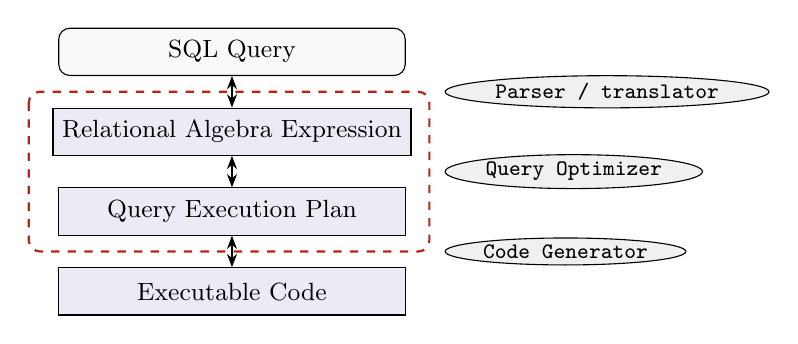
\begin{tikzpicture}[node distance=4mm, >=Stealth,
  box/.style={draw, fill=NavyBlue!8, minimum width=44mm, minimum height=6mm, font=\small},
  stepl/.style={draw, ellipse, fill=gray!12, font=\footnotesize\ttfamily, inner sep=1pt}]
\node[box, fill=gray!5, rounded corners] (sql) {SQL Query};
\node[box, below=of sql] (ra) {Relational Algebra Expression};
\node[box, below=of ra] (qep) {Query Execution Plan};
\node[box, below=of qep] (code) {Executable Code};
\draw[<->] (sql) -- (ra) node[midway, stepl, anchor=west, xshift=27mm] {Parser / translator};
\draw[<->] (ra) -- (qep) node[midway, stepl, anchor=west, xshift=27mm] {Query Optimizer};
\draw[<->] (qep) -- (code) node[midway, stepl, anchor=west, xshift=27mm] {Code Generator};
\draw[BrickRed, rounded corners, thick, dashed] ($(ra.north west)+(-3mm,2mm)$) rectangle ($(qep.south east)+(3mm,-2mm)$);
\end{tikzpicture}
\end{center}

\begin{itemize}
  \item \textbf{Relational algebra:} the basic set of operations for the relational model. Each operation takes one or two relations and returns a \textbf{new relation}, so operations can be \textbf{nested}. A sequence of RA operations is a \textbf{relational algebra expression}.
  \item Query processing has three steps: \textbf{(1) parsing and translation} (SQL $\to$ RA), \textbf{(2) optimization}, \textbf{(3) evaluation}.
\end{itemize}

%=====================================================================
\section{The Core Translation Rule}

\begin{keybox}[The one rule to remember]
\[
\underbrace{\sqlkw{SELECT}\ A_1,\dots,A_k}_{\pi}\ \ \underbrace{\sqlkw{FROM}\ R_1,\dots,R_n}_{\times}\ \ \underbrace{\sqlkw{WHERE}\ C}_{\sigma}
\quad\Longrightarrow\quad
\pi_{A_1,\dots,A_k}\big(\sigma_{C}(R_1 \times R_2 \times \dots \times R_n)\big)
\]
Evaluate from the \textbf{inside out}: \textbf{FROM} (product) $\rightarrow$ \textbf{WHERE} (selection) $\rightarrow$ \textbf{SELECT} (projection).
\end{keybox}

\begin{tabularx}{\linewidth}{@{}l l X@{}}
\toprule
\textbf{SQL clause / keyword} & \textbf{RA operator} & \textbf{Note}\\\midrule
\texttt{SELECT} list & $\pi$ (project) & \texttt{SELECT *} $\Rightarrow$ no $\pi$ at all\\
\texttt{FROM R, S} & $R \times S$ & comma = Cartesian product\\
\texttt{WHERE} condition & $\sigma$ (select) & \texttt{AND}$\to\wedge$, \texttt{OR}$\to\vee$, \texttt{NOT}$\to\neg$\\
\texttt{FROM R, S WHERE R.a = S.b} & $R \bowtie_{R.a=S.b} S$ & $\sigma$ over $\times$ = join\\
\texttt{JOIN \dots ON} $c$ / \texttt{USING} / \texttt{NATURAL JOIN} & $\bowtie_c$ / equi-join / $*$ or $\bowtie$ & \\
\texttt{LEFT / RIGHT / FULL OUTER JOIN} & $\lojoin$\ \ $\rojoin$\ \ $\fojoin$ & \\
\texttt{AS} (alias, column rename) & $\rho$ (rename) & \\
\texttt{UNION / INTERSECT / EXCEPT} & $\cup$\ \ $\cap$\ \ $-$ & operands must be union-compatible\\
\texttt{IN} (subquery) & join / semi-join $\ltimes$ & \\
\texttt{NOT IN}, \texttt{NOT EXISTS} & set difference $-$ & \\
``for \textbf{all} / every'' & division $\div$ & \\
\texttt{COUNT, SUM, AVG, MIN, MAX}, \texttt{GROUP BY} & $\agg$ or $\gamma$ (extended RA) & \texttt{HAVING} $\to$ $\sigma$ applied \emph{after} $\agg$\\
\texttt{DISTINCT} & (automatic) & RA is set-based: duplicates are always removed\\
\bottomrule
\end{tabularx}

\begin{warnbox}[SQL vs RA: sets and bags]
RA relations are \textbf{sets}, so $\pi$ removes duplicates automatically. SQL tables are \textbf{multisets (bags)}: \texttt{SELECT} keeps duplicates unless you write \texttt{DISTINCT}, and \texttt{UNION ALL} keeps duplicates while \texttt{UNION} removes them. For exam translations, treat \texttt{SELECT A} as $\pi_A$.
\end{warnbox}

\subsection*{Schemas used in the examples}
\begin{itemize}
  \item \textbf{University:} $\R{Student}(\underline{sid}, name, age, dept)$,\ \ $\R{Enroll}(\underline{sid, cid}, grade)$,\ \ $\R{Course}(\underline{cid}, cname)$.
  \item \small\textbf{COMPANY} (Elmasri, slide 192; keys underlined):\\
  EMPLOYEE(FNAME, MINIT, LNAME, \underline{SSN}, BDATE, ADDRESS, SEX, SALARY, SUPERSSN, DNO)\\
  DEPARTMENT(DNAME, \underline{DNUMBER}, MGRSSN, MGRSTARTDATE)\\
  DEPT\_LOCATIONS(\underline{DNUMBER, DLOCATION})\\
  PROJECT(PNAME, \underline{PNUMBER}, PLOCATION, DNUM)\\
  WORKS\_ON(\underline{ESSN, PNO}, HOURS)\\
  DEPENDENT(\underline{ESSN, DEPENDENT\_NAME}, SEX, BDATE, RELATIONSHIP)
\end{itemize}

%=====================================================================
\section{Unary Operations: $\sigma$, $\pi$, $\rho$}

\subsection{SELECT $\sigma$ (from \texttt{WHERE})}
$\sigma_{p}(r)$ keeps the \textbf{tuples (rows)} of $r$ that satisfy predicate $p$. Predicates use $=,\neq,<,\le,>,\ge$ joined by $\wedge,\vee,\neg$.
\begin{itemize}
  \item Result has the \textbf{same attributes} (degree) as $r$ and at most as many tuples: $|\sigma_p(r)| \le |r|$.
  \item \textbf{Commutative:} $\sigma_{c_1}(\sigma_{c_2}(R)) = \sigma_{c_2}(\sigma_{c_1}(R)) = \sigma_{c_1 \wedge c_2}(R)$ (cascade of $\sigma$).
  \item \textbf{Selection reduces rows, never columns.}
\end{itemize}

\begin{exbox}[Examples (slides 194--196, 199)]
\begin{tabularx}{\linewidth}{@{}p{0.36\linewidth} X@{}}
\texttt{SELECT * FROM Student WHERE dept = 'CSE';} & $\sigma_{dept='CSE'}(\R{Student})$ \quad (no $\pi$: \texttt{SELECT *})\\[2pt]
\texttt{SELECT * FROM EMPLOYEE WHERE SALARY > 30000;} & $\sigma_{SALARY>30000}(\R{EMPLOYEE})$\\[2pt]
\texttt{\dots\ WHERE Id > 3000 OR Hobby = 'hiking'} & $\sigma_{Id>3000\ \vee\ Hobby='hiking'}(\R{Person})$\\
\texttt{\dots\ WHERE Id > 3000 AND Id < 3999} & $\sigma_{Id>3000\ \wedge\ Id<3999}(\R{Person})$\\
\texttt{\dots\ WHERE NOT (Hobby = 'hiking')} & $\sigma_{\neg(Hobby='hiking')}(\R{Person}) \equiv \sigma_{Hobby\neq'hiking'}(\R{Person})$\\[2pt]
\texttt{\dots\ WHERE (DNO=4 AND SALARY>25000) OR (DNO=5 AND SALARY>30000)} & $\sigma_{(DNO=4 \wedge SALARY>25000)\ \vee\ (DNO=5 \wedge SALARY>30000)}(\R{EMPLOYEE})$\\
\end{tabularx}
Result of the last one on the COMPANY data: Franklin Wong (DNO 5, 40000), Jennifer Wallace (DNO 4, 43000), Ramesh Narayan (DNO 5, 38000).
\end{exbox}

\subsection{PROJECT $\pi$ (from the \texttt{SELECT} list)}
$\pi_{A_1,\dots,A_k}(r)$ keeps only the listed \textbf{attributes (columns)} and \textbf{removes duplicate tuples}.
\begin{itemize}
  \item $|\pi(r)| \le |r|$; if the list contains a key, $|\pi(r)| = |r|$.
  \item \textbf{Not} commutative, but a cascade collapses: $\pi_{L_1}(\pi_{L_2}(R)) = \pi_{L_1}(R)$ when $L_1 \subseteq L_2$.
\end{itemize}

\begin{exbox}[Example: duplicate elimination (slide 199, Fig.~7.8)]
$\pi_{LNAME,FNAME,SALARY}(\R{EMPLOYEE})$ returns all 8 employees. However, $\pi_{SEX,SALARY}(\R{EMPLOYEE})$ returns only \textbf{7} rows: Zelaya and English are both $\langle F, 25000\rangle$, so that tuple appears once. The SQL \texttt{SELECT SEX, SALARY FROM EMPLOYEE} would give 8 rows; \texttt{SELECT DISTINCT} gives 7.
\end{exbox}

\subsection{Selection + Projection together}
\begin{exbox}[Slide 198]
\texttt{SELECT name, age FROM Student WHERE dept = 'CSE';}
\[ \pi_{name,\,age}\big(\sigma_{dept='CSE'}(\R{Student})\big) \]
First $\sigma$ (row filter), then $\pi$ (column filter). Selection must come first here: if $\pi$ ran first, the attribute \texttt{dept} needed for filtering would be gone.
\end{exbox}

\subsection{RENAME $\rho$ and the assignment arrow $\leftarrow$}
\begin{itemize}
  \item $\rho_{S(B_1,\dots,B_n)}(R)$ renames relation $R$ to $S$ and its attributes to $B_1,\dots,B_n$. Also written $\rho_S(R)$ (relation only) or $\rho_{(B_1,\dots,B_n)}(R)$ (attributes only). The slides write $\rho_{a/b}(R)$ for ``rename attribute $b$ to $a$''.
  \item SQL \texttt{AS} aliases map to $\rho$, e.g.\ \texttt{FROM EMPLOYEE AS E} $\Rightarrow \rho_E(\R{EMPLOYEE})$.
  \item A long expression can be split into named steps with $\leftarrow$ (slide 201):
\end{itemize}
\begin{exbox}[In-line vs step-by-step]
\texttt{SELECT FNAME, LNAME, SALARY FROM EMPLOYEE WHERE DNO = 5;}
\[ \pi_{FNAME,LNAME,SALARY}\big(\sigma_{DNO=5}(\R{EMPLOYEE})\big) \]
\begin{gather*}
\R{DEP5\_EMPS} \leftarrow \sigma_{DNO=5}(\R{EMPLOYEE}) \\
\R{RESULT} \leftarrow \pi_{FNAME,LNAME,SALARY}(\R{DEP5\_EMPS})
\end{gather*}
Renaming the result's attributes: $\R{RESULT}(First, Last, Salary) \leftarrow \pi_{FNAME,LNAME,SALARY}(\R{DEP5\_EMPS})$.
\end{exbox}

\begin{exbox}[Multi-table SELECT-FROM-WHERE (slide 202)]
\texttt{SELECT movieTitle FROM StarsIn, MovieStar WHERE starName = name AND birthdate = 1960;}
\[ \pi_{movieTitle}\big(\sigma_{starName=name\ \wedge\ birthdate=1960}(\R{StarsIn} \times \R{MovieStar})\big) \]
This is exactly the core rule: FROM $\to\times$, WHERE $\to\sigma$, SELECT $\to\pi$.
\end{exbox}

%=====================================================================
\section{Set Operations: $\cup$, $\cap$, $-$ (from \texttt{UNION}, \texttt{INTERSECT}, \texttt{EXCEPT})}

\begin{keybox}[Union compatibility (required for $\cup$, $\cap$, $-$)]
$R(A_1,\dots,A_n)$ and $S(B_1,\dots,B_n)$ are union-compatible if they have the \textbf{same number of attributes} and $\mathrm{dom}(A_i) = \mathrm{dom}(B_i)$ for every $i$. The result takes the attribute names of the \textbf{first} relation. This is why we usually $\pi$ both sides to the same columns first.
\end{keybox}

\begin{tabularx}{\linewidth}{@{}l l l X@{}}
\toprule
\textbf{Op} & \textbf{SQL} & \textbf{RA} & \textbf{Result}\\\midrule
Union & \texttt{UNION} & $R \cup S$ & tuples in $R$ \textbf{or} $S$ (duplicates removed). Commutative, associative.\\
Intersection & \texttt{INTERSECT} & $R \cap S$ & tuples in \textbf{both}. Commutative, associative. Derived: $R \cap S = R - (R - S)$.\\
Difference & \texttt{EXCEPT} / \texttt{MINUS} & $R - S$ & tuples in $R$ but \textbf{not} in $S$. \textbf{Not} commutative: $R - S \neq S - R$.\\
\bottomrule
\end{tabularx}

\begin{exbox}[SQL $\to$ RA (slides 207, 211, 215)]
\begin{tabularx}{\linewidth}{@{}X X@{}}
\texttt{SELECT sid FROM Enroll UNION SELECT sid FROM Student;} & $\pi_{sid}(\R{Enroll}) \cup \pi_{sid}(\R{Student})$\\
\texttt{SELECT sid FROM Student INTERSECT SELECT sid FROM Enroll;} & $\pi_{sid}(\R{Student}) \cap \pi_{sid}(\R{Enroll})$ \ \ (students enrolled in something)\\
\texttt{SELECT sid FROM Student EXCEPT SELECT sid FROM Enroll;} & $\pi_{sid}(\R{Student}) - \pi_{sid}(\R{Enroll})$ \ \ (students \textbf{not} enrolled in any course)\\
\end{tabularx}
\end{exbox}

\begin{exbox}[Worked tables (slides 206, 210, 214, 216)]
\small
\begin{minipage}[t]{0.23\linewidth}\centering
\textbf{Course\_1}\\[1pt]
\begin{tabular}{cl}\toprule C\_id & C\_name\\\midrule 11 & Foundation C\\ 21 & C++\\ 31 & JAVA\\\bottomrule\end{tabular}
\end{minipage}\hfill
\begin{minipage}[t]{0.2\linewidth}\centering
\textbf{Course\_2}\\[1pt]
\begin{tabular}{cl}\toprule C\_id & C\_name\\\midrule 12 & Python\\ 21 & C++\\\bottomrule\end{tabular}
\end{minipage}\hfill
\begin{minipage}[t]{0.23\linewidth}\centering
\textbf{Course\_1 $\cup$ Course\_2}\\[1pt]
\begin{tabular}{cl}\toprule C\_id & C\_name\\\midrule 11 & Foundation C\\ 21 & C++\\ 31 & JAVA\\ 12 & Python\\\bottomrule\end{tabular}
\end{minipage}\hfill
\begin{minipage}[t]{0.23\linewidth}\centering
\textbf{Course\_1 $-$ Course\_2}\\[1pt]
\begin{tabular}{cl}\toprule C\_id & C\_name\\\midrule 11 & Foundation C\\ 31 & JAVA\\\bottomrule\end{tabular}\\[3pt]
\textbf{Course\_1 $\cap$ Course\_2}\\[1pt]
\begin{tabular}{cl}\toprule 21 & C++\\\bottomrule\end{tabular}
\end{minipage}

\medskip
\begin{minipage}[t]{0.18\linewidth}\centering
\textbf{A}\\[1pt]\begin{tabular}{ccc}\toprule k&x&y\\\midrule 1&A&2\\2&B&4\\3&C&6\\\bottomrule\end{tabular}
\end{minipage}\hfill
\begin{minipage}[t]{0.18\linewidth}\centering
\textbf{B}\\[1pt]\begin{tabular}{ccc}\toprule k&x&y\\\midrule 1&A&2\\4&D&8\\5&E&10\\\bottomrule\end{tabular}
\end{minipage}\hfill
\begin{minipage}[t]{0.16\linewidth}\centering
\textbf{A $\cap$ B}\\[1pt]\begin{tabular}{ccc}\toprule k&x&y\\\midrule 1&A&2\\\bottomrule\end{tabular}
\end{minipage}\hfill
\begin{minipage}[t]{0.4\linewidth}
\textbf{X1(Name, Age)} = \{Anoop 22, Saurav 22, Rakesh 20, Pritesh 19\}\\
\textbf{X2(Name, Age)} = \{Anoop 22, Anurag 23, Ganesh 21, Saurav 22, Rakesh 20\}\\
$X1 - X2 = $ \{Pritesh 19\}\\
$X2 - X1 = $ \{Anurag 23, Ganesh 21\} \ $\Rightarrow$ difference is \textbf{not commutative}.
\end{minipage}
\end{exbox}

%=====================================================================
\section{Cartesian Product $\times$ (from \texttt{FROM R, S} / \texttt{CROSS JOIN})}

$R \times S$ combines \textbf{every} tuple of $R$ with \textbf{every} tuple of $S$. No union compatibility needed.
\[
\text{degree}(R \times S) = n_R + n_S, \qquad |R \times S| = |R| \cdot |S|
\]
On its own it is rarely useful. It becomes meaningful when followed by a $\sigma$ that matches related tuples.

\begin{exbox}[Examples (slides 218, 220, 221)]
\texttt{SELECT * FROM A CROSS JOIN B;} with $A = \{1,2,3\}$, $B = \{x,y,z\}$ $\Rightarrow$ $A \times B$ has $3 \times 3 = 9$ tuples: (1,x), (1,y), (1,z), (2,x), \dots, (3,z).
$A1(Name, RollNo)$ with 2 rows $\times$ $A2(Name, RollNo)$ with 3 rows $\Rightarrow$ 6 rows, 4 columns.

\textbf{Step-by-step with product} (female employees and their dependents):
\begin{gather*}
\R{FEMALE\_EMPS} \leftarrow \sigma_{SEX='F'}(\R{EMPLOYEE}) \\
\R{EMPNAMES} \leftarrow \pi_{FNAME,LNAME,SSN}(\R{FEMALE\_EMPS})
\end{gather*}
\begin{gather*}
\R{EMP\_DEPENDENTS} \leftarrow \R{EMPNAMES} \times \R{DEPENDENT} \\
\R{ACTUAL\_DEPS} \leftarrow \sigma_{SSN=ESSN}(\R{EMP\_DEPENDENTS})
\end{gather*}
\[ \R{RESULT} \leftarrow \pi_{FNAME,LNAME,DEPENDENT\_NAME}(\R{ACTUAL\_DEPS}) \]
The last two steps ($\times$ then $\sigma_{SSN=ESSN}$) are exactly a join, $\R{EMPNAMES} \bowtie_{SSN=ESSN} \R{DEPENDENT}$.
\end{exbox}

%=====================================================================
\section{Joins $\bowtie$ (from \texttt{WHERE} join conditions or \texttt{JOIN \dots ON})}

\begin{keybox}[Join = product + selection]
\[ R \bowtie_{\theta} S \;=\; \sigma_{\theta}(R \times S) \]
Whenever an SQL \texttt{WHERE} clause compares attributes of \textbf{two different tables}, replace ``$\times$ then $\sigma$'' by $\bowtie$.
\end{keybox}

\begin{tabularx}{\linewidth}{@{}l l X@{}}
\toprule
\textbf{Join} & \textbf{Notation} & \textbf{Meaning}\\\midrule
Theta join (conditional) & $R \bowtie_{\theta} S$ & $\theta$ is any comparison $A\ op\ B$, $op \in \{=,\neq,<,\le,>,\ge\}$\\
Equi-join & $R \bowtie_{A=B} S$ & $\theta$ uses \textbf{only} $=$; both join columns stay in the result\\
Natural join & $R * S$ or $R \bowtie S$ & equi-join on \textbf{all same-named attributes}, keeping one copy of each\\
\bottomrule
\end{tabularx}

\subsection{Theta join}
\begin{exbox}[Customer $\bowtie_{Customer.cid > Order.oid}$ Order (slide 227)]
\small
\begin{minipage}[t]{0.25\linewidth}\centering
\textbf{Customer}\\\begin{tabular}{ccc}\toprule Cid&Cname&Age\\\midrule 101&Ajay&20\\102&Vijay&19\\103&Sita&21\\\bottomrule\end{tabular}
\end{minipage}\hfill
\begin{minipage}[t]{0.2\linewidth}\centering
\textbf{Order}\\\begin{tabular}{cc}\toprule Oid&Oname\\\midrule 101&Pizza\\101&Noodles\\103&Burger\\\bottomrule\end{tabular}
\end{minipage}\hfill
\begin{minipage}[t]{0.45\linewidth}\centering
\textbf{Result}\\\begin{tabular}{ccccc}\toprule Cid&Cname&Age&Oid&Oname\\\midrule 102&Vijay&19&101&Pizza\\102&Vijay&19&101&Noodles\\103&Sita&21&101&Pizza\\103&Sita&21&101&Noodles\\\bottomrule\end{tabular}
\end{minipage}

\smallskip
Ajay (101) is not $>$ any Oid. Nobody's Cid is $>$ 103, so Burger never appears.
\end{exbox}

\subsection{Equi-join}
\begin{exbox}[Slides 228, 229, 231, 232, 251]
\texttt{SELECT Student.name, Enroll.grade FROM Student, Enroll WHERE Student.sid = Enroll.sid;}
\[ \pi_{name,\,grade}\big(\R{Student} \bowtie_{Student.sid=Enroll.sid} \R{Enroll}\big) \qquad (\text{i.e. } \R{Student} \times \R{Enroll} + \sigma = \bowtie) \]
\texttt{SELECT name FROM Student, Enroll WHERE Student.sid = Enroll.sid AND grade = 'A';}
\[ \pi_{name}\big(\sigma_{grade='A'}(\R{Student} \bowtie_{Student.sid=Enroll.sid} \R{Enroll})\big) \]
Distinguish the two kinds of \texttt{WHERE} conditions: \textbf{join condition} ($Student.sid = Enroll.sid$, links two tables $\to \bowtie$) and \textbf{filter condition} ($grade = 'A'$, one table $\to \sigma$).

\texttt{SELECT * FROM Faculty, Offering WHERE Faculty.FacSSN = Offering.FacSSN;}
\[ \R{RESULT} \leftarrow \R{Faculty} \bowtie_{Faculty.FacSSN=Offering.FacSSN} \R{Offering} \]
joe (111-11-1111) matches offerings 1111 and 3333; sue matches 2222; sara matches none and is dropped. Both FacSSN columns appear in the result.

Sailors: $S1 \bowtie_{S1.sid=R1.sid} R1$ gives (22, dustin, 7, 45.0, 101, 10/10/96) and (58, rusty, 10, 35.0, 103, 11/12/96). The \texttt{sid} in R1 is a \textbf{foreign key} to S1.

Manager of each department: $\R{DEPT\_MGR} \leftarrow \R{DEPARTMENT} \bowtie_{MGRSSN=SSN} \R{EMPLOYEE}$ $\Rightarrow$ Research--Wong, Administration--Wallace, Headquarters--Borg.
\end{exbox}

\subsection{Natural join}
Only possible when the relations share an attribute with the \textbf{same name and type}. The duplicate column is dropped. If there is no common attribute, $R * S = R \times S$.
\begin{exbox}[Slides 235--237]
\small
\texttt{SELECT * FROM CLASS NATURAL JOIN CLASSINFO;} \ (or \texttt{INNER JOIN CLASSINFO USING (ID)}) \ $\Rightarrow\ \R{CLASS} * \R{CLASSINFO}$

\smallskip
\begin{minipage}[t]{0.2\linewidth}\centering
\textbf{CLASS}\\\begin{tabular}{cc}\toprule ID&NAME\\\midrule 1&AAA\\2&BBB\\4&DDD\\\bottomrule\end{tabular}
\end{minipage}\hfill
\begin{minipage}[t]{0.24\linewidth}\centering
\textbf{CLASSINFO}\\\begin{tabular}{cc}\toprule ID&ADDRESS\\\midrule 1&CHENNAI\\2&MUMBAI\\3&DELHI\\\bottomrule\end{tabular}
\end{minipage}\hfill
\begin{minipage}[t]{0.3\linewidth}\centering
\textbf{CLASS $*$ CLASSINFO}\\\begin{tabular}{ccc}\toprule ID&NAME&ADDRESS\\\midrule 1&AAA&CHENNAI\\2&BBB&MUMBAI\\\bottomrule\end{tabular}
\end{minipage}

\smallskip
$\R{Employee}(Name, EmpId, DeptName) * \R{Dept}(DeptName, Manager)$ joins on \texttt{DeptName}: Harry--George, Sally--Harriet, George--George, Harriet--Harriet. Production (Charles) has no employee and is dropped.

$r(A,B,C,D) \bowtie s(B,D,E)$ joins on \textbf{both} $B$ and $D$ and gives 5 tuples: $(\alpha,1,\alpha,a,\alpha)$, $(\alpha,1,\alpha,a,\gamma)$, $(\alpha,1,\gamma,a,\alpha)$, $(\alpha,1,\gamma,a,\gamma)$, $(\delta,2,\beta,b,\delta)$.

Textbook: $\R{PROJ\_DEPT} \leftarrow \R{PROJECT} * \rho_{(DNAME,DNUM,MGRSSN,MGRSTARTDATE)}(\R{DEPARTMENT})$. The rename makes \texttt{DNUMBER} into \texttt{DNUM} so that natural join finds the common attribute.
\end{exbox}

%=====================================================================
\section{Outer Joins $\lojoin$, $\rojoin$, $\fojoin$}

A normal (inner) join drops tuples that have no match. An \textbf{outer join} keeps them and pads the missing side with \textbf{NULL}.

\begin{tabularx}{\linewidth}{@{}l l l X@{}}
\toprule
\textbf{Join} & \textbf{RA} & \textbf{SQL} & \textbf{Keeps}\\\midrule
Left outer & $R \lojoin S$ & \texttt{LEFT OUTER JOIN} & all tuples of $R$ (left); unmatched $\to$ NULLs for $S$'s attributes\\
Right outer & $R \rojoin S$ & \texttt{RIGHT OUTER JOIN} & all tuples of $S$ (right); unmatched $\to$ NULLs for $R$'s attributes\\
Full outer & $R \fojoin S$ & \texttt{FULL OUTER JOIN} & all tuples of both sides\\
\bottomrule
\end{tabularx}

\begin{exbox}[CLASS / CLASSINFO on ID (slides 241, 245, 249)]
\small
\begin{minipage}[t]{0.31\linewidth}\centering
\textbf{Left:} $\R{CLASS} \lojoin \R{CLASSINFO}$\\
\begin{tabular}{ccc}\toprule ID&NAME&ADDRESS\\\midrule 1&AAA&CHENNAI\\2&BBB&MUMBAI\\4&DDD&NULL\\\bottomrule\end{tabular}
\end{minipage}\hfill
\begin{minipage}[t]{0.31\linewidth}\centering
\textbf{Right:} $\R{CLASS} \rojoin \R{CLASSINFO}$\\
\begin{tabular}{ccc}\toprule ID&NAME&ADDRESS\\\midrule 1&AAA&CHENNAI\\2&BBB&MUMBAI\\3&NULL&DELHI\\\bottomrule\end{tabular}
\end{minipage}\hfill
\begin{minipage}[t]{0.31\linewidth}\centering
\textbf{Full:} $\R{CLASS} \fojoin \R{CLASSINFO}$\\
\begin{tabular}{ccc}\toprule ID&NAME&ADDRESS\\\midrule 1&AAA&CHENNAI\\2&BBB&MUMBAI\\3&NULL&DELHI\\4&DDD&NULL\\\bottomrule\end{tabular}
\end{minipage}

\smallskip
SQL: \texttt{SELECT * FROM CLASS NATURAL LEFT | RIGHT | FULL OUTER JOIN CLASSINFO;}
\end{exbox}

\begin{exbox}[More slide examples (240, 242, 244, 246, 248, 250, 252)]
\begin{itemize}
  \item $\R{DEPT} \lojoin_{DEPT\_ID} \R{EMPLOYEE}$: Account has James and Rose, Design has Kathy and Marry, and Testing (30) has \textbf{no employee}, so it is kept with NULLs.
  \item $\R{EMPLOYEE} \rojoin_{DEPT\_ID} \R{DEPT}$: the same 4 matches, plus the row (NULL, NULL, NULL, 30, Testing).
  \item $\R{EMPLOYEE} \fojoin_{DEPT\_ID} \R{DEPT}$, where Alex (105) has DEPT\_ID 40 (no such department): the 4 matches, plus (105, Alex, 40, NULL, NULL), plus (NULL, NULL, NULL, 30, Testing).
  \item Table1(Products, Price) $\lojoin$ Table2(Products, Quantity): Kiwis 10, Onions 6, Tomatoes $\to$ Quantity NULL. Broccoli (right only) is dropped.
  \item Customers $\fojoin_{CustomerId}$ Orders: Shree--100, Basavaraj--300, Kalpana--NULL order, NULL customer--order 200 (CustomerId 4 does not exist).
  \item PARTS $\lojoin_{PROD\#}$ PRODUCTS keeps OIL (160) with NULL price. $\rojoin$ keeps product 505 (3.70) with NULL part. $\fojoin$ keeps both.
\end{itemize}
\end{exbox}

%=====================================================================
\section{Nested Queries and Query Blocks}

\begin{keybox}[Query block (slide 270)]
A \textbf{query block} is the basic unit that is translated into RA and optimized. It contains a \textbf{single} \texttt{SELECT-FROM-WHERE} expression, plus \texttt{GROUP BY} and \texttt{HAVING} if they are part of that block.
\begin{itemize}
  \item \textbf{Nested queries} inside a query are identified as \textbf{separate query blocks} and translated separately.
  \item \textbf{Aggregate operators} (\texttt{MAX}, \texttt{COUNT}, \dots) must be included in the \textbf{extended algebra} ($\agg$).
\end{itemize}
\end{keybox}

\begin{exbox}[Scalar subquery (slide 271)]
\begin{verbatim}
SELECT LNAME, FNAME
FROM   EMPLOYEE
WHERE  SALARY > ( SELECT MAX(SALARY) FROM EMPLOYEE WHERE DNO = 5 );
\end{verbatim}
The query is split into \textbf{two blocks}:

\begin{tabularx}{\linewidth}{@{}X X@{}}
\toprule
\textbf{Inner block} & \textbf{Outer block}\\\midrule
\texttt{SELECT MAX(SALARY) FROM EMPLOYEE WHERE DNO = 5} & \texttt{SELECT LNAME, FNAME FROM EMPLOYEE WHERE SALARY > }$c$\\[2pt]
$c \leftarrow \agg_{\,MAX\ SALARY}\big(\sigma_{DNO=5}(\R{EMPLOYEE})\big)$ & $\pi_{LNAME,FNAME}\big(\sigma_{SALARY>c}(\R{EMPLOYEE})\big)$\\
\bottomrule
\end{tabularx}
The inner block is \textbf{uncorrelated}: it is evaluated once and its result $c$ (a constant) is used in the outer block. On the COMPANY data, $c = 40000$ (Wong) and the answer is Wallace (43000) and Borg (55000).
\end{exbox}

\begin{exbox}[\texttt{IN} $\to$ join (slide 253)]
\texttt{SELECT name FROM Student WHERE sid IN (SELECT sid FROM Enroll);}

Step 1 (inner block): $\pi_{sid}(\R{Enroll})$.\qquad Step 2 (equivalent using a join):
\begin{gather*}
\pi_{name}\big(\R{Student} \bowtie \R{Enroll}\big) \\
\text{or exactly} \\
\pi_{name}\big(\R{Student} \ltimes \R{Enroll}\big)
\end{gather*}
\texttt{IN} is usually convertible into a \textbf{semi-join} $\ltimes$ (keeps the Student tuples that have at least one match, without adding Enroll's columns).
\end{exbox}

\begin{exbox}[\texttt{NOT IN} $\to$ difference (slide 254, corrected)]
\texttt{SELECT name FROM Student WHERE sid NOT IN (SELECT sid FROM Enroll);}
\[ \pi_{name}\Big(\R{Student} \bowtie \big(\pi_{sid}(\R{Student}) - \pi_{sid}(\R{Enroll})\big)\Big) \]
Find the \texttt{sid}s that are not enrolled (a difference of two union-compatible $\pi_{sid}$ relations), then join back to Student to get their names. An equivalent form is $\pi_{name}\big(\R{Student} - \pi_{sid,name,age,dept}(\R{Student} \bowtie \R{Enroll})\big)$. \texttt{NOT EXISTS} translates the same way.
\end{exbox}

%=====================================================================
\section{Division $\div$ (``for ALL'' queries)}

\begin{keybox}[Definition]
For $R(A, B)$ and $S(B)$, $R \div S$ returns the $A$-values that are paired in $R$ with \textbf{every} $B$-value in $S$:
\[ R \div S = \{\, t[A] \mid t \in R \ \wedge\ \forall s \in S\ \ \langle t[A], s\rangle \in R \,\} \]
In terms of basic operators:
\begin{gather*}
T_1 \leftarrow \pi_A(R), \\
T_2 \leftarrow \pi_A\big((T_1 \times S) - R\big), \\
R \div S = T_1 - T_2
\end{gather*}
$T_1 \times S$ is ``every candidate paired with every required value''. Subtracting $R$ leaves the missing pairs, so $T_2$ holds the candidates missing at least one value.
\end{keybox}

Use division when the question says \textbf{all}, \textbf{every} or \textbf{for all}: ``persons with an account in \emph{all} banks of a city'', ``students who have taken \emph{all} courses required to graduate''.

\begin{exbox}[Slide 256: A $\div$ B1, A $\div$ B2, A $\div$ B3]
\small
\begin{minipage}[t]{0.3\linewidth}
$A(x,y)$ = \{(x1,y1), (x1,y2), (x1,y3), (x1,y4), (x2,y1), (x2,y2), (x3,y2), (x4,y2), (x4,y4)\}
\end{minipage}\hfill
\begin{minipage}[t]{0.66\linewidth}
\begin{tabular}{@{}lll@{}}
\toprule
\textbf{Divisor} & \textbf{Result} & \textbf{Why}\\\midrule
$B1 = \{y2\}$ & $\{x1, x2, x3, x4\}$ & every $x$ has $y2$\\
$B2 = \{y2, y4\}$ & $\{x1, x4\}$ & only x1 and x4 have both $y2$ and $y4$\\
$B3 = \{y1, y2, y4\}$ & $\{x1\}$ & only x1 has all three\\
\bottomrule
\end{tabular}
\end{minipage}

\smallskip
Check $A \div B2$ with the formula: $T_1 = \{x1,x2,x3,x4\}$. $T_1 \times B2$ has 8 pairs. The pairs not in $A$ are (x2,y4) and (x3,y4), so $T_2 = \{x2, x3\}$ and $T_1 - T_2 = \{x1, x4\}$.
\end{exbox}

\begin{exbox}[Students enrolled in ALL courses (slide 257, SQL corrected)]
\begin{verbatim}
SELECT sid FROM Enroll
GROUP BY sid
HAVING COUNT(DISTINCT cid) = (SELECT COUNT(*) FROM Course);
\end{verbatim}
\[ \pi_{sid,\,cid}(\R{Enroll}) \div \pi_{cid}(\R{Course}) \]
Note: $\pi_{sid,cid}$ is needed first. Without it, \texttt{grade} would become part of the ``A'' side and break the division.

\textbf{Textbook (COMPANY):} employees who work on \emph{all} projects controlled by department 5:
\begin{gather*}
\R{DEPT5\_PROJS} \leftarrow \rho_{(PNO)}\big(\pi_{PNUMBER}(\sigma_{DNUM=5}(\R{PROJECT}))\big) \\
\R{EMP\_PROJ} \leftarrow \rho_{(SSN,PNO)}\big(\pi_{ESSN,PNO}(\R{WORKS\_ON})\big)
\end{gather*}
\begin{gather*}
\R{RESULT\_SSNS} \leftarrow \R{EMP\_PROJ} \div \R{DEPT5\_PROJS} \\
\R{RESULT} \leftarrow \pi_{LNAME,FNAME}(\R{RESULT\_SSNS} * \R{EMPLOYEE})
\end{gather*}
\end{exbox}

%=====================================================================
\section{Aggregate Functions and Grouping (Extended RA)}

Classical RA has \textbf{no} aggregation. The \textbf{extended} RA adds the aggregate function operator. Elmasri writes it $\agg$ (script F), and many other texts use $\gamma$:
\begin{gather*}
{}_{\langle\text{grouping attributes}\rangle}\ \agg_{\ \langle\text{function list}\rangle}(R) \\
\text{or} \\
\gamma_{\langle\text{grouping attrs}\rangle,\ \langle\text{function list}\rangle}(R)
\end{gather*}
Functions: \texttt{SUM}, \texttt{AVERAGE}, \texttt{MAXIMUM}, \texttt{MINIMUM}, \texttt{COUNT}. The attributes \textbf{before} $\agg$ are the \texttt{GROUP BY} columns. If there are none, the whole relation is one group and the result is a single tuple.

\begin{exbox}[SQL $\to$ extended RA (slides 259, 263)]
\begin{tabularx}{\linewidth}{@{}X X@{}}
\texttt{SELECT COUNT(*) FROM Student;} & $\gamma_{count(*)}(\R{Student})$ \ or \ $\agg_{COUNT\ sid}(\R{Student})$\\
\texttt{SELECT dept, COUNT(*) FROM Student GROUP BY dept;} & $\gamma_{dept,\ count(*)}(\R{Student})$ \ or \ ${}_{dept}\agg_{COUNT\ sid}(\R{Student})$\\
\texttt{SELECT MAX(Salary) FROM Employee;} & $\agg_{MAX\ Salary}(\R{Employee})$\\
\texttt{SELECT MIN(Salary) FROM Employee;} & $\agg_{MIN\ Salary}(\R{Employee})$\\
\texttt{SELECT SUM(Salary) FROM Employee;} & $\agg_{SUM\ Salary}(\R{Employee})$\\
\end{tabularx}
\end{exbox}

\begin{exbox}[GROUP BY + HAVING, and aggregates with a join]
\texttt{SELECT DNO, COUNT(*), AVG(SALARY) FROM EMPLOYEE GROUP BY DNO HAVING AVG(SALARY) > 30000;}
\begin{gather*}
\R{T} \leftarrow \rho_{(DNO,\,NO\_EMPS,\,AVG\_SAL)}\Big({}_{DNO}\,\agg_{\,COUNT\ SSN,\ AVERAGE\ SALARY}(\R{EMPLOYEE})\Big) \\
\R{RESULT} \leftarrow \sigma_{AVG\_SAL > 30000}(\R{T})
\end{gather*}
\texttt{WHERE} becomes a $\sigma$ \textbf{below} $\agg$ (it filters rows before grouping). \texttt{HAVING} becomes a $\sigma$ \textbf{above} $\agg$ (it filters groups after grouping). On the COMPANY data the groups are DNO 5 (4 employees, average 33250), DNO 4 (3, 31000) and DNO 1 (1, 55000). All three have an average above 30000.

\medskip
Slide 260: \texttt{SELECT country.country\_name, COUNT(city.lat), SUM(city.lat), AVG(city.lat), MIN(city.lat), MAX(city.lat) FROM city INNER JOIN country ON city.country\_id = country.id GROUP BY country.id, country.country\_name;}
\[ {}_{id,\ country\_name}\ \agg_{\ COUNT\ lat,\ SUM\ lat,\ AVERAGE\ lat,\ MIN\ lat,\ MAX\ lat}\big(\R{city} \bowtie_{city.country\_id = country.id} \R{country}\big) \]
followed by $\pi$ to drop \texttt{id}. USA has 2 cities, so its COUNT is 2 and its AVG (37.39) is SUM/2.
\end{exbox}

%=====================================================================
\section{Complete Translation: Query $Q2$, Query Tree and Query Graph}

\begin{exbox}[Q2 (slide 272)]
\emph{For every project located in `Stafford', list the project number, the controlling department number, and the department manager's last name, address and birth date.}
\begin{verbatim}
SELECT P.PNUMBER, P.DNUM, E.LNAME, E.ADDRESS, E.BDATE
FROM   PROJECT AS P, DEPARTMENT AS D, EMPLOYEE AS E
WHERE  P.DNUM = D.DNUMBER AND D.MGRSSN = E.SSN AND P.PLOCATION = 'Stafford';
\end{verbatim}
\textbf{Step 1: canonical (direct) translation} using the core rule:
\begin{gather*}
\pi_{L}\big(\sigma_{C}((P \times D) \times E)\big), \quad\text{where}\\
L = P.PNUMBER,\ P.DNUM,\ E.LNAME,\ E.ADDRESS,\ E.BDATE\\
C = P.DNUM=D.DNUMBER\ \wedge\ D.MGRSSN=E.SSN\ \wedge\ P.PLOCATION='Stafford'
\end{gather*}
\textbf{Step 2: sort the conditions.} $P.PLOCATION='Stafford'$ involves one table, so it is a filter ($\sigma$). $P.DNUM=D.DNUMBER$ and $D.MGRSSN=E.SSN$ each link two tables, so they are joins ($\bowtie$).

\textbf{Step 3: better RA expression} (textbook form):
\begin{multline*}
\pi_{PNUMBER,DNUM,LNAME,ADDRESS,BDATE}\Big(\big(\big(\sigma_{PLOCATION='Stafford'}(\R{PROJECT})\big)\\
\bowtie_{DNUM=DNUMBER} \R{DEPARTMENT}\big) \bowtie_{MGRSSN=SSN} \R{EMPLOYEE}\Big)
\end{multline*}
\end{exbox}

\begin{keybox}[Query tree vs query graph (slide 269)]
\begin{itemize}
  \item \textbf{Query tree:} a tree for an \textbf{RA expression}. \textbf{Leaves} are the input relations, and \textbf{internal nodes} are RA operations. Execution runs an internal node as soon as its operands are available, then replaces the node by the resulting relation. The root gives the answer. One query can have \textbf{many} query trees.
  \item \textbf{Query graph:} a graph for a \textbf{relational calculus} expression. Relation nodes are single circles and constant nodes are double circles. Selection and join conditions are edges, and the attributes to retrieve are shown in [ ] above each relation. It does \textbf{not} say which operation runs first, and there is only \textbf{one} graph per query.
\end{itemize}
\end{keybox}

\begin{center}
\begin{minipage}[t]{0.5\linewidth}\centering
\textbf{(a) Query tree for the Step-3 expression}\\[3pt]
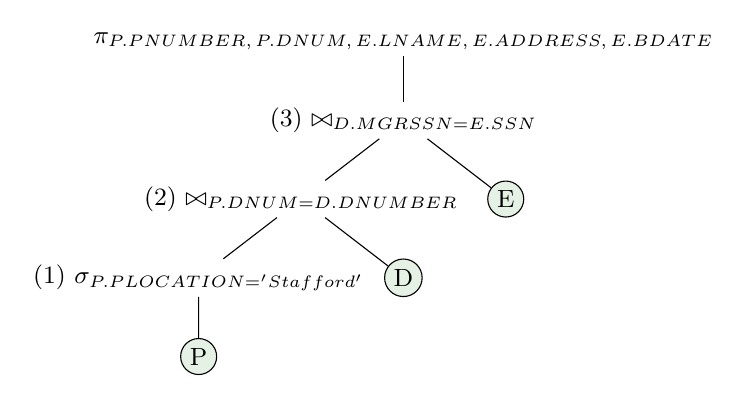
\begin{tikzpicture}[qt, level 1/.style={sibling distance=30mm}, level 2/.style={sibling distance=26mm}]
\node {$\pi_{P.PNUMBER,\,P.DNUM,\,E.LNAME,\,E.ADDRESS,\,E.BDATE}$}
  child {node {(3)\ $\bowtie_{D.MGRSSN=E.SSN}$}
    child {node {(2)\ $\bowtie_{P.DNUM=D.DNUMBER}$}
      child {node {(1)\ $\sigma_{P.PLOCATION='Stafford'}$}
        child {node[relnode] {P}}}
      child {node[relnode] {D}}}
    child {node[relnode] {E}}};
\end{tikzpicture}
\end{minipage}\hfill
\begin{minipage}[t]{0.48\linewidth}\centering
\textbf{(b) Initial (canonical) query tree}\\[3pt]
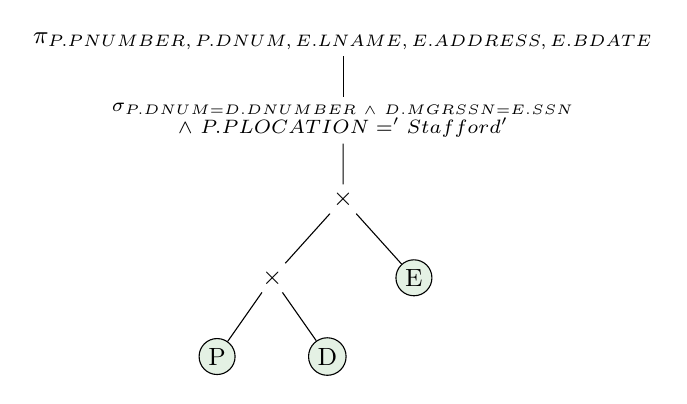
\begin{tikzpicture}[qt, level 3/.style={sibling distance=18mm}, level 4/.style={sibling distance=14mm}]
\node {$\pi_{P.PNUMBER,\,P.DNUM,\,E.LNAME,\,E.ADDRESS,\,E.BDATE}$}
  child {node[align=center, font=\scriptsize] {$\sigma_{P.DNUM=D.DNUMBER\ \wedge\ D.MGRSSN=E.SSN}$\\$\wedge\ P.PLOCATION='Stafford'$}
    child {node {$\times$}
      child {node {$\times$}
        child {node[relnode] {P}}
        child {node[relnode] {D}}}
      child {node[relnode] {E}}}};
\end{tikzpicture}
\end{minipage}
\end{center}

\begin{center}
\textbf{(c) Query graph for Q2}\\[2pt]
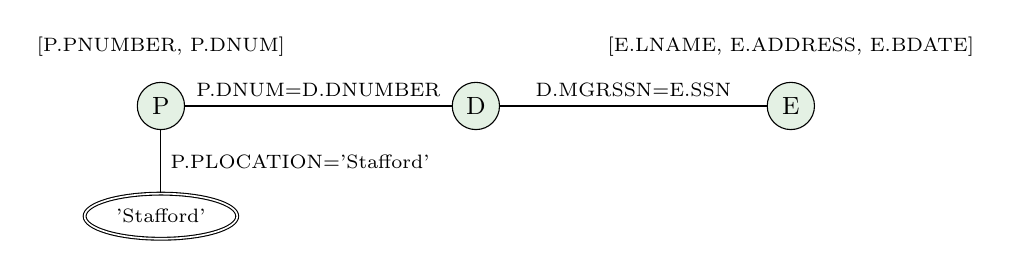
\begin{tikzpicture}[font=\small]
\node[relnode, minimum size=6mm] (P) at (0,0) {P};
\node[relnode, minimum size=6mm] (D) at (4,0) {D};
\node[relnode, minimum size=6mm] (E) at (8,0) {E};
\node[draw, double, ellipse, font=\scriptsize] (S) at (0,-1.4) {'Stafford'};
\draw (P) -- node[above, font=\scriptsize] {P.DNUM=D.DNUMBER} (D);
\draw (D) -- node[above, font=\scriptsize] {D.MGRSSN=E.SSN} (E);
\draw (P) -- node[right, font=\scriptsize] {P.PLOCATION='Stafford'} (S);
\node[above=2mm of P, font=\scriptsize] {[P.PNUMBER, P.DNUM]};
\node[above=2mm of E, font=\scriptsize] {[E.LNAME, E.ADDRESS, E.BDATE]};
\end{tikzpicture}
\end{center}

The \textbf{canonical tree (b)} is what the parser produces directly from SQL: $\times$ of the FROM tables, one big $\sigma$, then $\pi$. It is correct but very expensive, because $P \times D \times E$ is huge. Heuristic optimization (the next topic) rewrites it into trees like (a): push $\sigma$ down, turn $\sigma$ over $\times$ into $\bowtie$, and push $\pi$ down.

\begin{exbox}[Another canonical translation (slide 276)]
\texttt{SELECT LNAME FROM EMPLOYEE, WORKS\_ON, PROJECT WHERE PNAME = 'Aquarius' AND PNUMBER = PNO AND ESSN = SSN AND BDATE > '1957-12-31';}
\begin{gather*}
\text{Canonical: }\ \pi_{LNAME}\big(\sigma_{C}(\R{EMPLOYEE} \times \R{WORKS\_ON} \times \R{PROJECT})\big),\\
C = PNAME='Aquarius'\ \wedge\ PNUMBER=PNO\ \wedge\ ESSN=SSN\ \wedge\ BDATE>\text{'1957-12-31'}
\end{gather*}
\begin{multline*}
\text{With joins: }\ \pi_{LNAME}\Big(\big(\sigma_{PNAME='Aquarius'}(\R{PROJECT}) \bowtie_{PNUMBER=PNO} \R{WORKS\_ON}\big)\\
\bowtie_{ESSN=SSN} \sigma_{BDATE>\text{'1957-12-31'}}(\R{EMPLOYEE})\Big)
\end{multline*}
\end{exbox}

%=====================================================================
\section{Step-by-Step Recipe and Practice}

\begin{keybox}[How to translate any SQL query]
\begin{enumerate}
  \item \textbf{Split into query blocks.} Translate each nested subquery separately, innermost first.
  \item \textbf{FROM:} write the tables (use $\rho$ for aliases), combined with $\times$.
  \item \textbf{WHERE:} sort each condition. If it links two tables, it is a \textbf{join condition} ($\bowtie$). If it involves one table, it is a \textbf{filter} ($\sigma$, applied to that table as early as possible).
  \item \textbf{Subquery predicates:} \texttt{IN}/\texttt{EXISTS} $\to$ join or semi-join. \texttt{NOT IN}/\texttt{NOT EXISTS} $\to$ difference. ``All'' $\to$ division. A scalar subquery becomes a constant $c$ computed by $\agg$.
  \item \textbf{GROUP BY / aggregates:} ${}_{G}\agg_{F}$. \textbf{HAVING} is a $\sigma$ on top of it.
  \item \textbf{SELECT list:} $\pi$ at the top. Skip it for \texttt{SELECT *}. Use $\rho$ for \texttt{AS} column names.
  \item \textbf{UNION / INTERSECT / EXCEPT:} translate each side, make them union-compatible with $\pi$, and combine with $\cup$, $\cap$ or $-$.
\end{enumerate}
\end{keybox}

\begin{exbox}[Practice (COMPANY schema), with answers]
\textbf{1.} Names of employees in the `Research' department.\\
\texttt{SELECT FNAME, LNAME, ADDRESS FROM EMPLOYEE, DEPARTMENT WHERE DNAME = 'Research' AND DNUMBER = DNO;}
\[ \pi_{FNAME,LNAME,ADDRESS}\big(\sigma_{DNAME='Research'}(\R{DEPARTMENT}) \bowtie_{DNUMBER=DNO} \R{EMPLOYEE}\big) \]
\textbf{2.} Employees who work on project `ProductX'.\\
\texttt{SELECT E.FNAME, E.LNAME FROM EMPLOYEE E, WORKS\_ON W, PROJECT P WHERE E.SSN = W.ESSN AND W.PNO = P.PNUMBER AND P.PNAME = 'ProductX';}
\begin{multline*}
\pi_{FNAME,LNAME}\Big(\big(\sigma_{PNAME='ProductX'}(\R{PROJECT}) \bowtie_{PNUMBER=PNO} \R{WORKS\_ON}\big)\\
\bowtie_{ESSN=SSN} \R{EMPLOYEE}\Big)
\end{multline*}
\textbf{3.} Employees with \emph{no} dependents.\\
\texttt{SELECT FNAME, LNAME FROM EMPLOYEE WHERE SSN NOT IN (SELECT ESSN FROM DEPENDENT);}
\begin{gather*}
\R{NO\_DEP} \leftarrow \pi_{SSN}(\R{EMPLOYEE}) - \rho_{(SSN)}\big(\pi_{ESSN}(\R{DEPENDENT})\big) \\
\R{RESULT} \leftarrow \pi_{FNAME,LNAME}(\R{NO\_DEP} * \R{EMPLOYEE})
\end{gather*}
\textbf{4.} Project numbers that involve an employee named `Smith', either as a worker or as the department manager.\\
\texttt{(SELECT PNO FROM WORKS\_ON, EMPLOYEE WHERE ESSN = SSN AND LNAME = 'Smith') UNION (SELECT PNUMBER FROM PROJECT, DEPARTMENT, EMPLOYEE WHERE DNUM = DNUMBER AND MGRSSN = SSN AND LNAME = 'Smith');}
\begin{multline*}
\pi_{PNO}\big(\R{WORKS\_ON} \bowtie_{ESSN=SSN} \sigma_{LNAME='Smith'}(\R{EMPLOYEE})\big)\\
\cup\ \pi_{PNUMBER}\Big(\R{PROJECT} \bowtie_{DNUM=DNUMBER}\\
\big(\R{DEPARTMENT} \bowtie_{MGRSSN=SSN} \sigma_{LNAME='Smith'}(\R{EMPLOYEE})\big)\Big)
\end{multline*}
\textbf{5.} Number of employees and average salary per department.\\
\texttt{SELECT DNO, COUNT(*), AVG(SALARY) FROM EMPLOYEE GROUP BY DNO;}
\[ {}_{DNO}\,\agg_{\,COUNT\ SSN,\ AVERAGE\ SALARY}(\R{EMPLOYEE}) \]

\textbf{6.} Every employee with their supervisor's name (self-join with rename).\\
\texttt{SELECT E.LNAME, S.LNAME FROM EMPLOYEE AS E, EMPLOYEE AS S WHERE E.SUPERSSN = S.SSN;}
\[ \pi_{E.LNAME,\,S.LNAME}\big(\rho_E(\R{EMPLOYEE}) \bowtie_{E.SUPERSSN=S.SSN} \rho_S(\R{EMPLOYEE})\big) \]
\end{exbox}

%=====================================================================
\section{Errors in the Slides}

\begin{warnbox}[Corrections]
\small
\begin{tabularx}{\linewidth}{@{}l X@{}}
\toprule
\textbf{Slide} & \textbf{Issue $\to$ correct version}\\\midrule
194 & ``$SALARY > 30{,}000\ (\R{EMPLOYEE})$'' is missing the $\sigma$, and the output text says `300000'. Correct: $\sigma_{SALARY>30000}(\R{EMPLOYEE})$.\\
197, 201, 219 & The $\pi$ and $\sigma$ symbols and the $\leftarrow$ arrows are lost in the slide text. Correct forms: $\pi_{LNAME,FNAME,SALARY}(\R{EMPLOYEE})$ and $\R{DEP5\_EMPS} \leftarrow \sigma_{DNO=5}(\R{EMPLOYEE})$.\\
212 & The result of EMP\_TEST INTERSECT EMP\_DESIGN is labelled ``UNION''. It is the \textbf{intersection} (only 104 Kathy).\\
228 & The condition $Student.sid = Enroll.sid$ is labelled a theta join. It is correct but more precisely an \textbf{equi-join} (a theta join that uses only $=$).\\
231 & ``Faculty.FacSSM'' $\to$ Faculty.\textbf{FacSSN}.\\
249 & The full outer join result is missing the ID column values and labels CLASSINFO's second column NAME. Correct result: (1, AAA, CHENNAI), (2, BBB, MUMBAI), (3, NULL, DELHI), (4, DDD, NULL).\\
250 & The OrderDate values in the result table do not match the Orders input table. Only the NULL pattern is meaningful.\\
253 & $\pi_{name}(\R{Student} \bowtie \R{Enroll})$ matches \texttt{IN} as a set. The exact operator is the semi-join $\R{Student} \ltimes \R{Enroll}$.\\
254 & $\R{Student} - (\R{Student} \bowtie \R{Enroll})$ is \textbf{invalid}: the two sides are not union-compatible (the join has extra attributes \texttt{cid} and \texttt{grade}). Correct: $\pi_{name}\big(\R{Student} \bowtie (\pi_{sid}(\R{Student}) - \pi_{sid}(\R{Enroll}))\big)$.\\
257 & \texttt{HAVING COUNT(cid)} should be \texttt{COUNT(DISTINCT cid)} for the SQL to match $\div$. It also assumes every \texttt{cid} in Enroll exists in Course.\\
272 & ``P.NUMBER'' $\to$ P.\textbf{PNUMBER}; ``‘ STAFFORD ’'' has stray spaces. The RA line on the slide has lost its $\pi$, $\sigma$ and $\bowtie$ symbols (see Q2 above).\\
276 & ``PNMUBER'' $\to$ \textbf{PNUMBER}.\\
\bottomrule
\end{tabularx}
\end{warnbox}

%=====================================================================
\section{Quick Revision}

\begin{keybox}[Symbols (slide 264) and the SQL they come from]
\small
\begin{tabularx}{\linewidth}{@{}l l X@{}}
$\sigma$ (sigma) & SELECT (selection) & \texttt{WHERE} (rows)\\
$\pi$ (pi) & PROJECT & \texttt{SELECT} list (columns, duplicates removed)\\
$\rho$ (rho) & RENAME & \texttt{AS}\\
$\times$ (times) & CARTESIAN PRODUCT & \texttt{FROM R, S}, \texttt{CROSS JOIN}\\
$\bowtie$ (bow-tie) & JOIN (theta / equi / natural $*$) & \texttt{WHERE R.a = S.b}, \texttt{JOIN \dots ON}, \texttt{NATURAL JOIN}\\
$\lojoin\ \rojoin\ \fojoin$ & OUTER JOINS & \texttt{LEFT / RIGHT / FULL OUTER JOIN}\\
$\cup$ (cup) \ $\cap$ (cap) \ $-$ (minus) & UNION, INTERSECTION, DIFFERENCE & \texttt{UNION}, \texttt{INTERSECT}, \texttt{EXCEPT}\\
$\div$ & DIVISION & ``for all'' / \texttt{NOT EXISTS \dots NOT EXISTS} / \texttt{COUNT = COUNT}\\
$\agg$ or $\gamma$ & AGGREGATE (extended RA) & \texttt{COUNT/SUM/AVG/MIN/MAX}, \texttt{GROUP BY}\\
\end{tabularx}
\end{keybox}

\begin{itemize}
  \item \textbf{Operator classes (slide 262).} \textbf{Basic unary:} $\sigma, \pi, \rho$. \textbf{Basic binary:} $\cup, \times, -$. \textbf{Derived:} $\bowtie$ ($=\sigma(\times)$), $\cap$ ($=R-(R-S)$), $\div$ (from $\pi, \times, -$). The complete set is $\{\sigma, \pi, \cup, \rho, -, \times\}$.
  \item \textbf{Core rule:} $\pi_{\text{SELECT}}(\sigma_{\text{WHERE}}(\times_{\text{FROM}}))$ is the \textbf{canonical} form; turning $\sigma$ over $\times$ into $\bowtie$ is the first improvement.
  \item \textbf{Selection before projection} whenever $\pi$ would drop an attribute that $\sigma$ needs.
  \item $|R \times S| = |R|\cdot|S|$; $\cup$, $\cap$, $-$ need union compatibility; $-$ is not commutative.
  \item Natural join: common attributes with the same name, one copy kept. With no common attribute, it equals $\times$.
  \item \textbf{Query block} = one SELECT-FROM-WHERE (+ GROUP BY/HAVING). Nested queries are separate blocks. Aggregates need extended RA.
  \item \textbf{WHERE} $\to$ $\sigma$ below $\agg$; \textbf{HAVING} $\to$ $\sigma$ above $\agg$.
  \item \textbf{Query tree:} leaves = relations, internal nodes = operators; many per query. \textbf{Query graph:} for relational calculus, no execution order, one per query.
\end{itemize}

\end{document}
